\documentclass[11pt, a4paper]{article}

\usepackage{graphicx}
\usepackage{amsmath}

\title{Explanation and causality}
\author{Daniel Gustafsson}
\date{September 2021}

\begin{document}
\maketitle

\section{Two research studies}

\subsection{To comment or not to comment?}
I do not think that we can draw the conclusion that comments improve code from this study.
This study is based on a single specific problem, maybe a conclusion could be drawn that for this specific problem
or this specific type of problem, programmers who uses comments specific to the given style guide writes better programs.

Another problem with the conclusion is that all group A students followed a specific style guide with their comments,
but the do not specifically state that the comments have to follow that same style guide.

If we want to compare results from two different groups we want the groups to be random, in this case the students
chose themselves which group to join which causes bias in the results.

We also do not know how many students partook in the study and how many joined each group, the possibility exists that
there were many students in group A and few in group B which gave group A a bigger chance to produce good programs and
in term distorting the results.

I suggest that the students are randomly assigned to the groups, provided a set of different problems to solve and students in
group A are free to choose any style guide for their comments.

\subsection{Java v Haskell}
I still do not think the given conclusion can be drawn. This study is better than the last in that the students are randomly
assigned but there is still just one specific problem. The specific problem could very well be much easier to solve using
object oriented program and thus be biased.

There is also a possibility that the students coursework is largely using Java and rarely using Haskell which also would
distort the results. The students could simply be more comfortable coding in Java than Haskell.

Another possibility is that Haskell is a slow language and that there are other functional programming languages that run faster,
maybe even faster than Java (or any object oriented language).

I suggest that the student in the group C can choose any functional language and students in group D can choose any \textit{non}
functional language. I also suggest that the student write programs to solve a set of different problems.

\section{Zipf's law}

\begin{figure}[h]
	% GNUPLOT: LaTeX picture with Postscript
\begingroup
  \makeatletter
  \providecommand\color[2][]{%
    \GenericError{(gnuplot) \space\space\space\@spaces}{%
      Package color not loaded in conjunction with
      terminal option `colourtext'%
    }{See the gnuplot documentation for explanation.%
    }{Either use 'blacktext' in gnuplot or load the package
      color.sty in LaTeX.}%
    \renewcommand\color[2][]{}%
  }%
  \providecommand\includegraphics[2][]{%
    \GenericError{(gnuplot) \space\space\space\@spaces}{%
      Package graphicx or graphics not loaded%
    }{See the gnuplot documentation for explanation.%
    }{The gnuplot epslatex terminal needs graphicx.sty or graphics.sty.}%
    \renewcommand\includegraphics[2][]{}%
  }%
  \providecommand\rotatebox[2]{#2}%
  \@ifundefined{ifGPcolor}{%
    \newif\ifGPcolor
    \GPcolorfalse
  }{}%
  \@ifundefined{ifGPblacktext}{%
    \newif\ifGPblacktext
    \GPblacktexttrue
  }{}%
  % define a \g@addto@macro without @ in the name:
  \let\gplgaddtomacro\g@addto@macro
  % define empty templates for all commands taking text:
  \gdef\gplbacktext{}%
  \gdef\gplfronttext{}%
  \makeatother
  \ifGPblacktext
    % no textcolor at all
    \def\colorrgb#1{}%
    \def\colorgray#1{}%
  \else
    % gray or color?
    \ifGPcolor
      \def\colorrgb#1{\color[rgb]{#1}}%
      \def\colorgray#1{\color[gray]{#1}}%
      \expandafter\def\csname LTw\endcsname{\color{white}}%
      \expandafter\def\csname LTb\endcsname{\color{black}}%
      \expandafter\def\csname LTa\endcsname{\color{black}}%
      \expandafter\def\csname LT0\endcsname{\color[rgb]{1,0,0}}%
      \expandafter\def\csname LT1\endcsname{\color[rgb]{0,1,0}}%
      \expandafter\def\csname LT2\endcsname{\color[rgb]{0,0,1}}%
      \expandafter\def\csname LT3\endcsname{\color[rgb]{1,0,1}}%
      \expandafter\def\csname LT4\endcsname{\color[rgb]{0,1,1}}%
      \expandafter\def\csname LT5\endcsname{\color[rgb]{1,1,0}}%
      \expandafter\def\csname LT6\endcsname{\color[rgb]{0,0,0}}%
      \expandafter\def\csname LT7\endcsname{\color[rgb]{1,0.3,0}}%
      \expandafter\def\csname LT8\endcsname{\color[rgb]{0.5,0.5,0.5}}%
    \else
      % gray
      \def\colorrgb#1{\color{black}}%
      \def\colorgray#1{\color[gray]{#1}}%
      \expandafter\def\csname LTw\endcsname{\color{white}}%
      \expandafter\def\csname LTb\endcsname{\color{black}}%
      \expandafter\def\csname LTa\endcsname{\color{black}}%
      \expandafter\def\csname LT0\endcsname{\color{black}}%
      \expandafter\def\csname LT1\endcsname{\color{black}}%
      \expandafter\def\csname LT2\endcsname{\color{black}}%
      \expandafter\def\csname LT3\endcsname{\color{black}}%
      \expandafter\def\csname LT4\endcsname{\color{black}}%
      \expandafter\def\csname LT5\endcsname{\color{black}}%
      \expandafter\def\csname LT6\endcsname{\color{black}}%
      \expandafter\def\csname LT7\endcsname{\color{black}}%
      \expandafter\def\csname LT8\endcsname{\color{black}}%
    \fi
  \fi
    \setlength{\unitlength}{0.0500bp}%
    \ifx\gptboxheight\undefined%
      \newlength{\gptboxheight}%
      \newlength{\gptboxwidth}%
      \newsavebox{\gptboxtext}%
    \fi%
    \setlength{\fboxrule}{0.5pt}%
    \setlength{\fboxsep}{1pt}%
\begin{picture}(6802.00,4534.00)%
    \gplgaddtomacro\gplbacktext{%
      \csname LTb\endcsname%%
      \put(946,704){\makebox(0,0)[r]{\strut{}$1$}}%
      \put(946,1907){\makebox(0,0)[r]{\strut{}$10$}}%
      \put(946,3110){\makebox(0,0)[r]{\strut{}$100$}}%
      \put(946,4313){\makebox(0,0)[r]{\strut{}$1000$}}%
      \put(1078,484){\makebox(0,0){\strut{}$1000$}}%
      \put(2854,484){\makebox(0,0){\strut{}$10000$}}%
      \put(4629,484){\makebox(0,0){\strut{}$100000$}}%
      \put(6405,484){\makebox(0,0){\strut{}$1\times10^{6}$}}%
    }%
    \gplgaddtomacro\gplfronttext{%
      \csname LTb\endcsname%%
      \put(209,2508){\rotatebox{-270}{\makebox(0,0){\strut{}log(Average payoff)}}}%
      \put(3741,154){\makebox(0,0){\strut{}log(Number of simulations)}}%
      \csname LTb\endcsname%%
      \put(5418,4140){\makebox(0,0)[r]{\strut{}Data}}%
    }%
    \gplbacktext
    \put(0,0){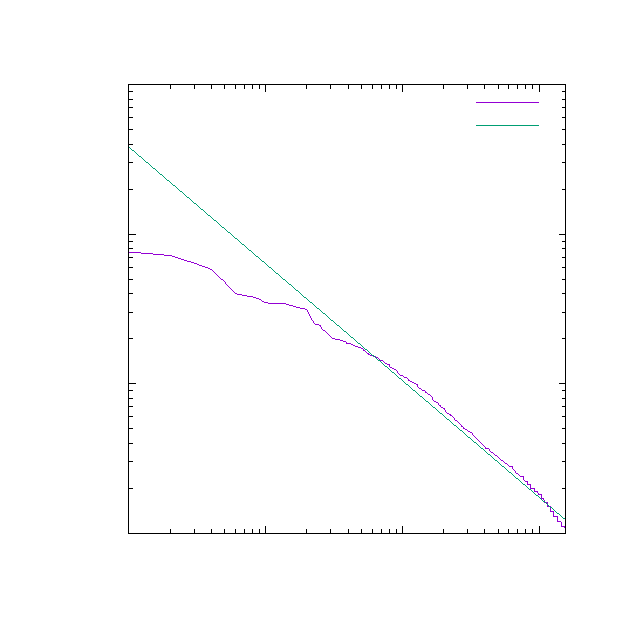
\includegraphics{plot}}%
    \gplfronttext
  \end{picture}%
\endgroup

\end{figure}

\bibliographystyle{amsplain}
\bibliography{hw3.bib}

\end{document}